\documentclass[11pt,a4paper]{article}
\usepackage[margin=19mm,headheight=14pt]{geometry}
\usepackage[T1]{fontenc}
\usepackage{lmodern}
\usepackage{amsmath,amssymb,booktabs,array,graphicx}
\usepackage{xcolor,tikz,fancyhdr,hyperref}
\usetikzlibrary{arrows.meta,calc,patterns,angles,quotes}
\definecolor{ink}{HTML}{18334A}
\definecolor{teal}{HTML}{008D91}
\definecolor{blue}{HTML}{2674B8}
\definecolor{orange}{HTML}{D67826}
\definecolor{muted}{HTML}{536878}
\definecolor{pale}{HTML}{EAF5F5}
\hypersetup{colorlinks=true,urlcolor=blue,linkcolor=blue,
pdftitle={Muon coincidences in the fridge: an illustrated integration guide},
pdfauthor={Cosmic-geant analysis}}
\pagestyle{fancy}
\fancyhf{}
\fancyhead[L]{\small\color{muted}CRYO DETECTOR \quad / \quad GEOMETRIC MUON ACCEPTANCE}
\fancyfoot[L]{\small\color{muted}Illustrated calculation \quad $\cdot$ \quad 24 September 2026}
\fancyfoot[R]{\small\thepage}
\renewcommand{\headrulewidth}{0.3pt}
\setlength{\parindent}{0pt}
\setlength{\parskip}{6pt}
\setlength{\abovedisplayskip}{8pt}
\setlength{\belowdisplayskip}{8pt}
\newcommand{\pageheading}[2]{{\color{teal}\small\bfseries #1}\par
{\color{ink}\LARGE\bfseries #2}\par\vspace{5pt}}
\newcommand{\note}[1]{\par\noindent\colorbox{pale}{\parbox{\dimexpr\linewidth-2\fboxsep\relax}{\vspace{4pt}#1\vspace{4pt}}}\par}
\newcommand{\captiontext}[1]{{\small\color{muted}#1}\par}
\tikzset{ray/.style={-{Latex[length=2.5mm]},very thick,blue},
dim/.style={<->,>=Latex,thin,muted},
block/.style={draw=teal,fill=teal!12,thick},
lab/.style={font=\small,text=ink,align=center}}
\begin{document}

\pageheading{01 / THE DETECTOR}{What is a coincidence?}
One muon must cross \textbf{both plastic blocks}. Each block produces light,
read out by its own SiPM. The SiPMs measure the light; their small area does not
set the muon collection area.

\begin{center}
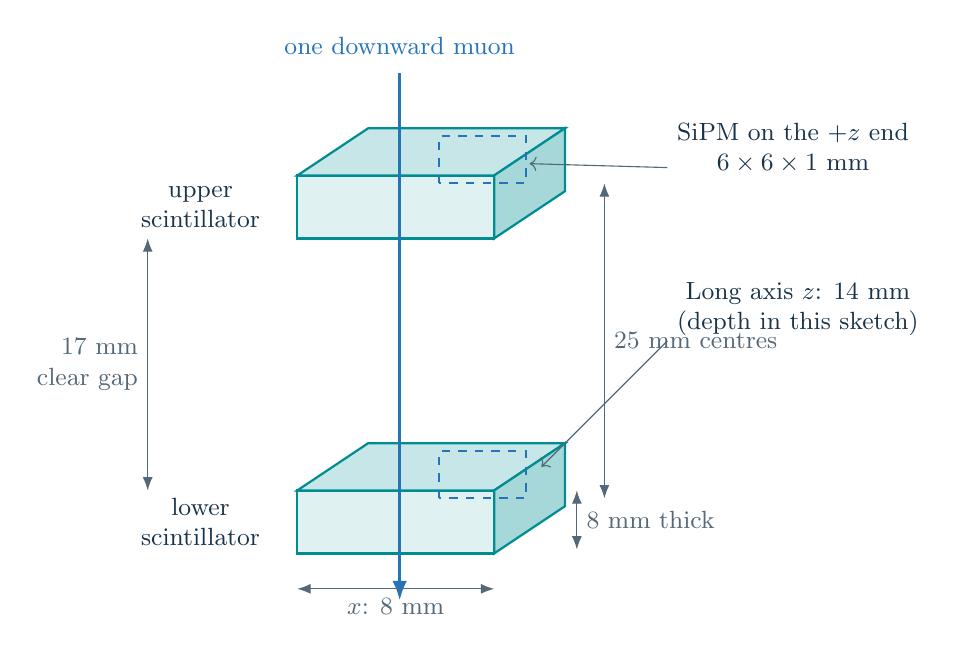
\begin{tikzpicture}[x=1cm,y=1cm]
\foreach \y/\name in {0/lower,4.0/upper}{
  \filldraw[block] (0,\y) rectangle (2.5,\y+.8);
  \filldraw[draw=teal,fill=teal!22,thick]
    (0,\y+.8)--(.9,\y+1.4)--(3.4,\y+1.4)--(2.5,\y+.8)--cycle;
  \filldraw[draw=teal,fill=teal!35,thick]
    (2.5,\y)--(3.4,\y+.6)--(3.4,\y+1.4)--(2.5,\y+.8)--cycle;
  \draw[blue,thick,dashed] (1.8,\y+.7) rectangle (2.9,\y+1.3);
  \node[lab,anchor=east] at (-.35,\y+.4) {\name\\scintillator};
}
\draw[ray] (1.3,6.1)--(1.3,-.6);
\node[lab,text=blue] at (1.3,6.45) {one downward muon};
\draw[dim] (3.9,.7)--(3.9,4.7) node[midway,right,font=\small] {25 mm centres};
\draw[dim] (-1.9,.8)--(-1.9,4.0) node[midway,left,font=\small,align=right] {17 mm\\clear gap};
\draw[dim] (0,-.45)--(2.5,-.45) node[midway,below,font=\small] {$x$: 8 mm};
\draw[dim] (3.55,.05)--(3.55,.8) node[midway,right,font=\small] {8 mm thick};
\node[lab,anchor=west] at (4.7,5.15) {SiPM on the $+z$ end\\$6\times6\times1$ mm};
\draw[muted,->] (4.7,4.9)--(2.95,4.95);
\node[lab,anchor=west] at (4.7,3.1) {Long axis $z$: 14 mm\\(depth in this sketch)};
\draw[muted,->] (4.7,2.7)--(3.1,1.1);
\end{tikzpicture}
\end{center}
\captiontext{Schematic 3D view, not to scale. Dashed blue marks indicate the far-end SiPMs;
their 0.5 mm coupling gaps are not resolved. The vertical axis is $y$.}

The footprint seen by a vertical muon is $8\times14$ mm, not $8\times8$ mm.
The blocks are 8 mm thick vertically:
\[
\underbrace{d}_{25\ {\rm mm}}
=\frac{\underbrace{h}_{8\ {\rm mm}}}{2}
+\underbrace{g}_{17\ {\rm mm}}
+\frac{h}{2}.
\]
We use $a=0.8$ cm along $x$, $b=1.4$ cm along $z$, $h=0.8$ cm
vertically, and centre separation $d=2.5$ cm.

\note{\textbf{Three different questions:}
Does a ray cross both blocks? Does it travel far enough inside each to make
a detectable pulse? How many such rays arrive in this lab per hour?}

\newpage
\pageheading{02 / TRACKS AND OVERLAP}{Corners count---until the signal is too small}
\begin{center}
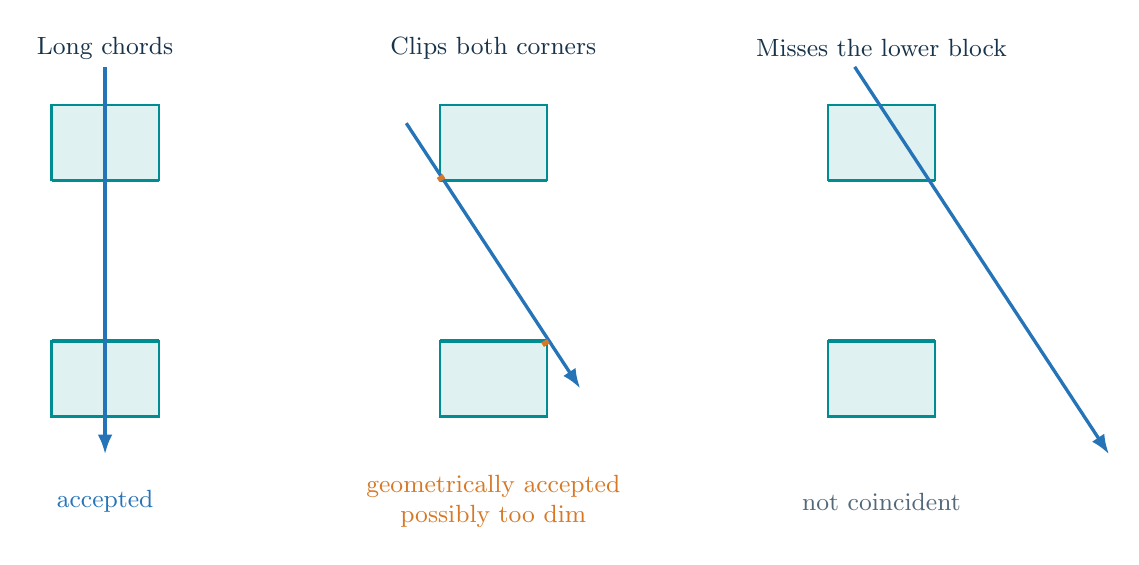
\begin{tikzpicture}[x=.17cm,y=.12cm]
\foreach \shift/\title in {0/Long chords,29/Clips both corners,58/Misses the lower block}{
\begin{scope}[xshift=\shift*.17cm]
\draw[block] (-4,21) rectangle (4,29);
\draw[block] (-4,-4) rectangle (4,4);
\draw[teal,very thick] (-4,21)--(4,21);
\draw[teal,very thick] (-4,4)--(4,4);
\node[lab] at (0,35) {\title};
\end{scope}}
\draw[ray] (0,33)--(0,-8);
\draw[ray] (22.5,27.04)--(35.5,-1.04);
\draw[orange,line width=2.5pt] (25,21.447)--(25.2,21);
\draw[orange,line width=2.5pt] (32.8,4)--(33,3.553);
\draw[ray] (56,33)--(75,-8);
\node[lab,text=blue] at (0,-13) {accepted};
\node[lab,text=orange] at (29,-13) {geometrically accepted\\possibly too dim};
\node[lab,text=muted] at (58,-13) {not coincident};
\end{tikzpicture}
\end{center}
\captiontext{Side projections; proportions simplified. Orange marks show the short
segments inside the blocks. The full calculation includes both horizontal coordinates.}

For identical, aligned blocks, any straight ray crossing both volumes must
cross the two \textbf{facing surfaces}. A ray that has already left their
shared horizontal footprint cannot turn back into it. Consequently, integrating
over these two faces includes the full 3D blocks, including side entries.

For a fixed direction, shift one facing rectangle onto the plane of the other.
Their overlap is the region of starting positions that can hit both:
\begin{center}
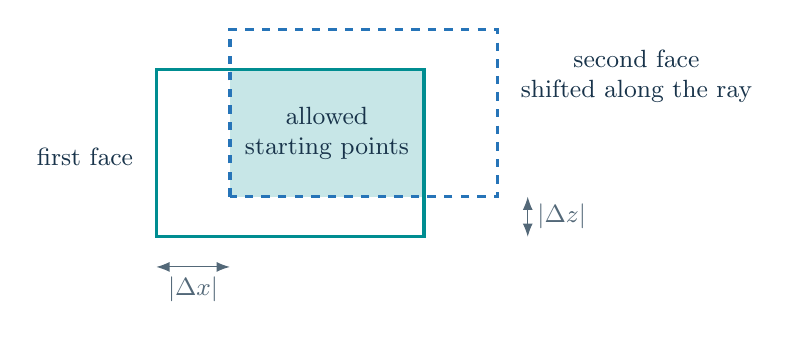
\begin{tikzpicture}[scale=.85]
\fill[teal!22] (1.1,.6) rectangle (4,2.5);
\draw[teal,very thick] (0,0) rectangle (4,2.5);
\draw[blue,very thick,dashed] (1.1,.6) rectangle (5.1,3.1);
\node[lab] at (2.55,1.55) {allowed\\starting points};
\node[lab,anchor=east] at (-.2,1.2) {first face};
\node[lab,anchor=west] at (5.3,2.4) {second face\\shifted along the ray};
\draw[dim] (0,-.45)--(1.1,-.45) node[midway,below,font=\small] {$|\Delta x|$};
\draw[dim] (5.55,0)--(5.55,.6) node[midway,right,font=\small] {$|\Delta z|$};
\end{tikzpicture}
\end{center}
Writing $\theta$ for zenith and $\phi$ for azimuth,
\[
\Delta x=g\tan\theta\cos\phi,\qquad
\Delta z=g\tan\theta\sin\phi,
\]
\[
\boxed{A_{\rm both}(\theta,\phi)
=[a-|\Delta x|]_+\,[b-|\Delta z|]_+},\qquad [r]_+=\max(0,r).
\]
\note{Using the \textbf{17 mm facing gap} gives 11.73 coincidences/hour.
Using 25 mm instead would count crossings of the centre planes, giving only
6.39/hour and missing valid corner-clipping tracks.}

\newpage
\pageheading{03 / SOLID ANGLE}{Adding up all incoming directions}
\begin{center}
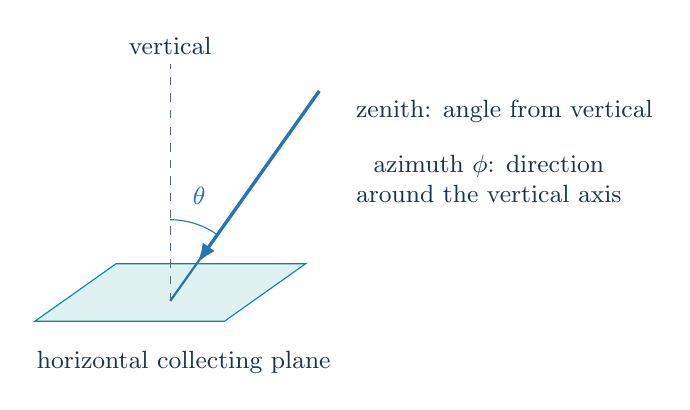
\begin{tikzpicture}[scale=.86]
\draw[fill=teal!12,draw=teal] (-2,-.3)--(.8,-.3)--(2,.55)--(-.8,.55)--cycle;
\coordinate (O) at (0,0);
\draw[dashed,muted] (0,0)--(0,3.5) node[above,lab] {vertical};
\draw[blue,thick] (0,0)--(2.2,3.1);
\draw[ray] (2.2,3.1)--(.4,.56);
\draw[blue] (0,1.2) arc[start angle=90,end angle=54.6,radius=1.2];
\node[lab,text=blue] at (.43,1.55) {$\theta$};
\node[lab,anchor=west] at (2.6,2.8) {zenith: angle from vertical};
\node[lab,anchor=west] at (2.6,1.8) {azimuth $\phi$: direction\\around the vertical axis};
\node[lab] at (.2,-.9) {horizontal collecting plane};
\end{tikzpicture}
\end{center}
\textbf{Specific intensity.} Let $I(\theta,\phi)$ be the muon flux measured on a
surface held \emph{perpendicular to the arrival direction}: muons per unit time,
per unit perpendicular area, per unit solid angle. This is a property of the
incoming muons alone --- it says nothing about the shape, distance, or extent of
whatever produced them (see the note below). The sea-level reference model is
$I(\theta,\phi)=I_0\cos^n\theta$ with $n=2$, uniform in $\phi$.

\textbf{Deriving $d\Omega=\sin\theta\,d\theta\,d\phi$.} On the unit sphere, the
circle of fixed zenith angle $\theta$ (a line of constant latitude) has radius
$\sin\theta$ about the vertical axis: a step $d\phi$ covers arc length
$\sin\theta\,d\phi$ along it. A step $d\theta$ covers arc length $d\theta$ along
a meridian, and meridians always meet latitude circles at right angles. The
patch bounded by $d\theta$ and $d\phi$ is therefore a right-angled rectangle of
area
\[
d\Omega=(d\theta)(\sin\theta\,d\phi)=\sin\theta\,d\theta\,d\phi,
\]
equal to its solid angle because the sphere has unit radius. Check: the upper
hemisphere must subtend $2\pi$ sr,
\[
\int_0^{2\pi}\!\!\int_0^{\pi/2}\sin\theta\,d\theta\,d\phi
=2\pi\big[-\cos\theta\big]_0^{\pi/2}=2\pi.\ \checkmark
\]

\textbf{The $\cos\theta$ projection factor.} $I$ is defined per unit area held
\emph{perpendicular} to the ray, but the collecting surface here is horizontal.
A horizontal patch of area $dA$, viewed along a ray arriving at zenith angle
$\theta$, presents a foreshortened area $dA\cos\theta$ to that ray --- its
shadow on the plane perpendicular to the ray. Equivalently, for current density
$\mathbf J$ along the ray and horizontal unit normal $\hat n$, the flux through
the horizontal surface is $\mathbf J\cdot\hat n=|\mathbf J|\cos\theta$. This
discards no crossings; every muon that reaches the plane is still counted. It
only converts a flux quoted per perpendicular area into a flux per horizontal
area, for the same stream of muons.

\textbf{Assembling and solving the integral.} Multiply intensity, projection,
and solid angle, then integrate over the hemisphere:
\[
F=\int_0^{2\pi}\!\!\int_0^{\pi/2}
 I_0\cos^n\theta\,\underbrace{\cos\theta}_{\text{projection}}\,
 \underbrace{\sin\theta\,d\theta\,d\phi}_{d\Omega}.
\]
The $\phi$ integral is trivial (uniform integrand, giving $2\pi$). Substituting
$u=\cos\theta$, $du=-\sin\theta\,d\theta$ (so $\theta:0\to\pi/2$ maps to
$u:1\to0$) turns the $\theta$ integral into
\[
\int_0^{\pi/2}\cos^{n+1}\theta\sin\theta\,d\theta
=\int_0^1 u^{n+1}\,du=\frac{1}{n+2},
\]
so
\[
\boxed{F=\frac{2\pi I_0}{n+2}.}
\]
For $F=1\ {\rm cm^{-2}\,min^{-1}}$ and $n=2$,
$I_0=2/\pi=0.63662\ {\rm cm^{-2}\,min^{-1}\,sr^{-1}}$.

\note{\textbf{Why the source geometry does not appear here:} $I(\theta,\phi)$ is
defined at the detector, purely as a function of arrival direction, so this
integral is unaffected by whether muons originate from a distant point, an
extended atmospheric production layer, or CRY's finite generation plane --- the
only requirement is the far-field approximation, that this source region is
much larger than the detector so $I(\theta,\phi)$ does not vary across the lab.
The production geometry instead sets the \emph{shape} of $\cos^n\theta$ itself
(a longer slant path at large $\theta$ loses more muons to decay before reaching
sea level); this document takes that shape as an empirical reference law rather
than re-deriving it from atmospheric transport.}

\textbf{The rate integral.} Replace the fixed unit area above with a chosen
direction-dependent selection $A(\theta,\phi)$ (one block, both, or a signal
cut) and integrate the same way:
\[
\boxed{R[A]=60I_0\int_0^{2\pi}\!\!\int_0^{\pi/2}
 A(\theta,\phi)\cos^{n+1}\theta\sin\theta\,d\theta\,d\phi.}
\]
The factor 60 converts minutes to hours; areas here are in cm$^2$. The
projection is already accounted for by the extra $\cos\theta$ folded into
$\cos^{n+1}\theta$, so $A(\theta,\phi)$ itself is a plain any-crossing indicator
area (the overlap area from page 2) --- it does not need its own projection
factor. At every direction, the integral weights that accepted area by how
frequently muons arrive from that direction.

\textbf{Side entry for one block.} The projected area includes its top and sides:
\[
A_{\rm one}=ab+hb\tan\theta|\cos\phi|+ha\tan\theta|\sin\phi|.
\]
Inserting $A_{\rm one}$ gives \textbf{120/hour per full block}. Inserting $ab$
counts only crossings of one horizontal face: \textbf{67.2/hour}.
Inserting $A_{\rm both}$ gives \textbf{11.73/hour}.

\note{\textbf{Numerical, not just symbolic:} the notebook evaluates these integrals
as weighted sums over angles. Increasing quadrature order from 64 to 512
leaves the uncut result at 11.72636/hour.}

\newpage
\pageheading{04 / SIGNAL THRESHOLD}{A pulse cut becomes a minimum chord}
Assume pulse amplitude is proportional to path length:
\[
V=V_{\rm ref}\frac{\ell}{\ell_{\rm ref}},
\qquad
L_{\min}=\ell_{\rm ref}\frac{V_{\rm th}}{V_{\rm ref}}.
\]
\textbf{Conditional calibration:} if 20.5 mV corresponds to an 8 mm path,
a 1 mV threshold requires
\[
\boxed{L_{\min}=8\,\frac{1}{20.5}=0.39024\ {\rm mm}
\quad\text{inside each block}.}
\]
A mean pulse height from mixed tracks does not, by itself, establish this calibration.

\begin{center}
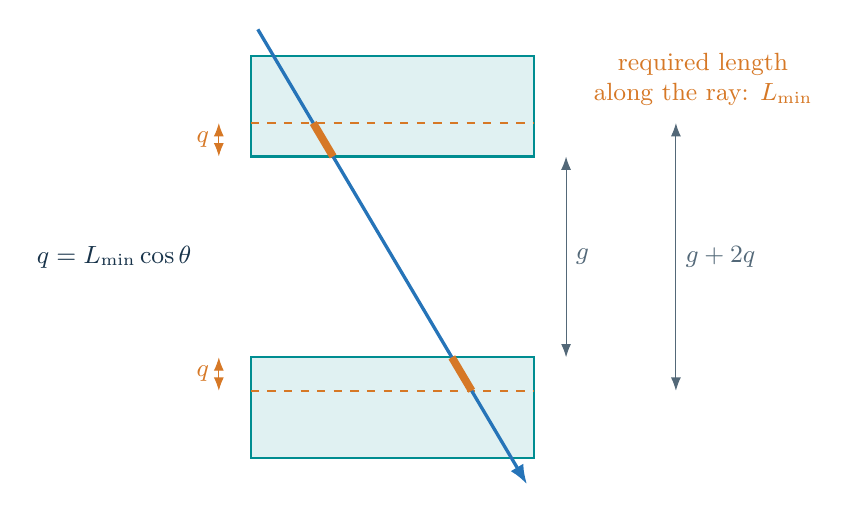
\begin{tikzpicture}[x=.9cm,y=.85cm]
\draw[block] (0,4.5) rectangle (4,6);
\draw[block] (0,0) rectangle (4,1.5);
\draw[orange,dashed,thick] (0,5.0)--(4,5.0);
\draw[orange,dashed,thick] (0,1.0)--(4,1.0);
\draw[ray] (.1,6.4)--(3.9,-.4);
\draw[orange,line width=2.8pt] (.882,5)--(1.162,4.5);
\draw[orange,line width=2.8pt] (2.838,1.5)--(3.118,1);
\draw[dim] (4.45,1.5)--(4.45,4.5) node[midway,right,font=\small] {$g$};
\draw[dim,orange] (-.45,4.5)--(-.45,5) node[midway,left,font=\small] {$q$};
\draw[dim,orange] (-.45,1)--(-.45,1.5) node[midway,left,font=\small] {$q$};
\draw[dim] (6.0,1)--(6.0,5) node[midway,right,font=\small] {$g+2q$};
\node[lab,anchor=east] at (-.7,3) {$q=L_{\min}\cos\theta$};
\node[lab,anchor=west,text=orange] at (4.7,5.65) {required length\\along the ray: $L_{\min}$};
\end{tikzpicture}
\end{center}
\captiontext{Required depths exaggerated for visibility. Orange segments have length
$L_{\min}$ along the ray; their vertical projections have length $q$.}

The accepted ray must reach the dashed plane inside \emph{each} block.
Replace the gap by $s=g+2L_{\min}\cos\theta$ in the overlap formula:
\[
A_{\rm cut}
=[a-s\tan\theta|\cos\phi|]_+\,
 [b-s\tan\theta|\sin\phi|]_+.
\]
Set $A_{\rm cut}=0$ if $L_{\min}\cos\theta>h$.
The same angular integral then gives \textbf{11.04167/hour}: a \textbf{5.84\% loss}.

\note{The amplitude ratio is 4.88\%, but the count loss is 5.84\%.
The latter comes from the distribution of paths through \emph{both} blocks.
Energy-loss and photon fluctuations are not included in this sharp-cut model.}

\newpage
\pageheading{05 / EXPECTED RATE}{From geometry to the lab}
\begin{center}
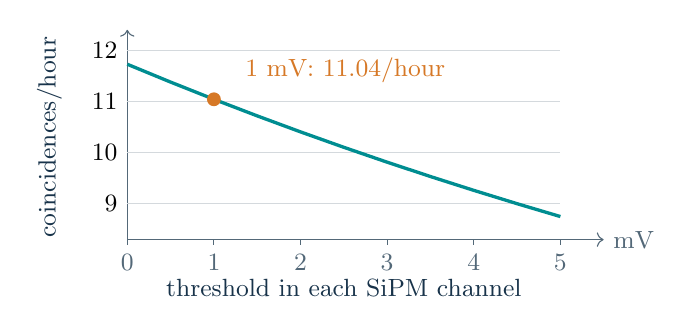
\begin{tikzpicture}[x=1.1cm,y=.65cm]
\draw[->,muted] (0,8.3)--(5.5,8.3) node[right,font=\small] {mV};
\draw[->,muted] (0,8.3)--(0,12.4);
\foreach \x in {0,1,2,3,4,5}
 {\draw[muted] (\x,8.3)--(\x,8.2) node[below,font=\small] {\x};}
\foreach \y in {9,10,11,12}
 {\draw[muted!25] (0,\y)--(5,\y);
  \node[left,font=\small] at (0,\y) {\y};}
\draw[teal,very thick] plot coordinates {
(0,11.726364) (.5,11.377800) (1,11.041671) (1.5,10.717549)
(2,10.405010) (2.5,10.103645) (3,9.813050) (3.5,9.532835)
(4,9.262618) (4.5,9.002028) (5,8.750707)};
\fill[orange] (1,11.041671) circle[radius=2.5pt];
\node[lab,anchor=west,text=orange] at (1.25,11.6) {1 mV: 11.04/hour};
\node[lab] at (2.5,7.35) {threshold in each SiPM channel};
\node[lab,rotate=90] at (-.9,10.3) {coincidences/hour};
\end{tikzpicture}
\end{center}
\captiontext{Numerically integrated threshold curve before environmental scaling;
assumes 20.5 mV for an 8 mm path. It is not a measured spectrum.}

\textbf{The measured environmental factor.}
The 17 July cryo-detector logbook records the same Luxium detector in two locations:
24.4 muons/min in our lab, and 18 muons/min beneath the dilution fridge in
David's lab. Matilda used the rounded transmission 0.74.
\[
T=\frac{18}{24.4}=0.73770,\qquad 1-T=26.23\%.
\]
Treating $T$ as independent of angle gives
\[
R_{\rm lab}=60I_0\int T A_{\rm cut}\cos^{n+1}\theta\,d\Omega
=T R_{\rm cut}.
\]

\begin{center}
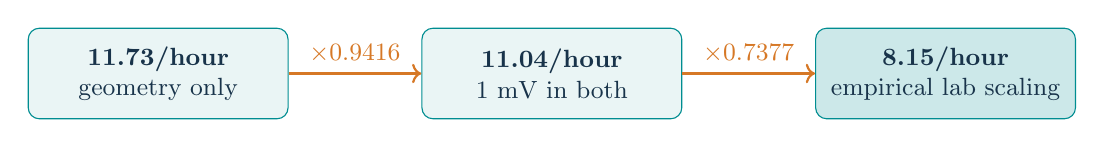
\begin{tikzpicture}[node distance=1cm]
\node[draw=teal,rounded corners,fill=pale,minimum width=3.3cm,minimum height=1.15cm,lab]
 (a) at (0,0) {\textbf{11.73/hour}\\geometry only};
\node[draw=teal,rounded corners,fill=pale,minimum width=3.3cm,minimum height=1.15cm,lab]
 (b) at (5,0) {\textbf{11.04/hour}\\1 mV in both};
\node[draw=teal,rounded corners,fill=teal!20,minimum width=3.3cm,minimum height=1.15cm,lab]
 (c) at (10,0) {\textbf{8.15/hour}\\empirical lab scaling};
\draw[->,thick,orange] (a)--(b) node[midway,above,font=\small] {$\times0.9416$};
\draw[->,thick,orange] (b)--(c) node[midway,above,font=\small] {$\times0.7377$};
\end{tikzpicture}
\end{center}

This suggests a mean interval of about \textbf{7.4 minutes} between accepted
coincidences under these assumptions.

\note{\textbf{What the factor means:} this is a relative measurement between
locations, not an isolated measurement of fridge absorption. Applying it to
the reference flux assumes the reference lab is representative, the detector
efficiency was stable, and the ratio transfers to our angular acceptance.
Do not also apply it to a flux already measured at the detector.}

Matilda's 30 August 100-million-event simulation reports 8.05/hour after its
0.74 scaling. That is close, but it used a \textbf{20 mV threshold with a different
photon-to-voltage calibration}, so the agreement is not a like-for-like validation.

\newpage
\pageheading{06 / CHECKS AND SOURCES}{The full 3D calculation behind the drawings}
For a ray passing through a reference point $(x,z)$ with angles $(\theta,\phi)$,
let $\ell_{\rm u}$ and $\ell_{\rm l}$ be its actual chord lengths in the upper
and lower blocks. Define
\[
S=\mathbf{1}[\ell_{\rm u}>0,\ \ell_{\rm l}>0]\,
  \mathbf{1}[\ell_{\rm u}\ge L_{\min},\ \ell_{\rm l}\ge L_{\min}].
\]
The unreduced position-and-angle integral is
\[
R=60I_0\int_0^{2\pi}\int_0^{\pi/2}\int_{\mathbb{R}^2}
 S(x,z,\theta,\phi)\cos^{n+1}\theta\sin\theta\,
 dx\,dz\,d\theta\,d\phi.
\]
For each direction, $\int S\,dx\,dz$ is exactly the allowed overlap area used
on the previous pages. Thus the surface method is a reduction of the 3D
ray calculation, not an assumption that the scintillators are thin sheets.

\textbf{Independent numerical check.} The notebook samples one million rays,
intersects them with each 3D box, measures both chords, and integrates the
accept/reject result. Sampled $\mu=\cos\theta$ has density
$p(\mu)=(n+2)\mu^{n+1}$, including projection and solid-angle weighting.
\begin{center}
\begin{tabular}{lrrr}
\toprule
Selection & Angular quadrature & 3D Monte Carlo & GEANT4 \\
 & /hour & /hour & /hour \\
\midrule
Both blocks, no threshold & 11.73 & $11.72\pm0.03$ & $11.7\pm0.3$ \\
Both above threshold & 11.04 & $11.04\pm0.02$ & $10.9\pm0.3$ \\
$\times\,T$ lab transmission & 8.145 & $8.146\pm0.018$ & $8.0\pm0.2$ \\
\bottomrule
\end{tabular}
\end{center}
Errors are rounded to one significant figure, or two if the leading digit is 1
(Taylor's rule), and each central value to the matching decimal place. The
\textbf{angular quadrature} and \textbf{3D Monte Carlo} columns are both this
document's own geometric model (ray-crossing only, no photon transport), so
they share $T=0.7377$; their errors are one-standard-error Monte Carlo
integration errors, \textbf{not} uncertainty estimates for the real detector.

The \textbf{GEANT4} column is a genuinely different calculation: Matilda's
30 August 100-million-event simulation with full optical-photon transport
(\texttt{cryo\_detector/logbooks/2026-08-30.md}, lines 168--219), using a
20 mV threshold with a different photon-to-voltage calibration and the
rounded $T=0.74$ --- \textbf{not} the same threshold or transmission value as
the other two columns, so treat same-row entries as analogous stages of the
calculation, not matched inputs. Its raw counts, over 10{,}309 minutes of
muon-clock live time, were 2010 any-photon double coincidences (no voltage
cut) and 1869 above the 20 mV cut; errors above are Poisson,
$\sigma=\sqrt{N}\times(60/10309\ {\rm min})$, propagated through $T=0.74$ on
the last row using the logbook's own quoted Poisson band.

None of these errors say anything about $T$ itself: the 24.4/18 mu/min Luxium
comparison behind this document's $T=0.7377$ only has rates logged
(\texttt{cryo\_detector/logbooks/2026-07-17.md}, line 64), with no raw counts
or run duration recorded, so $T$'s own statistical uncertainty cannot be
estimated from available records for either column.

\textbf{Remaining physical inputs.}
The model omits light-collection variation, energy-loss and photon statistics,
timing-window efficiency, dead time, and direction-dependent transport.
A pulse-height calibration measured on this system already includes SiPM
photon-detection efficiency; do not multiply by that efficiency a second time.

\textbf{Sources and reproducibility}
\begin{enumerate}
\setlength{\itemsep}{2pt}
\item Geometry: \texttt{geometry/dilutiondetector\_simplified\_fridge.gdml}
in the \texttt{dilutiondetector} branch of \texttt{cosmic-geant}.
\item \href{https://pdgweb.lbl.gov/2022/reviews/rpp2022-rev-cosmic-rays.pdf}
{Particle Data Group, Cosmic Rays (2022), section 30.3.1}:
reference sea-level flux and approximate $\cos^2\theta$ angular law.
\item Local cryo-detector logbooks:
\texttt{cryo\_detector/logbooks/2026-07-17.md}, lines 58--68
(Luxium measurement); \texttt{2026-08-06.md}, lines 34--37
(application); \texttt{2026-08-30.md}, lines 185--205 (100M result).
\item Executable derivation: \texttt{geometric\_muon\_rate.ipynb};
command-line integration: \texttt{geometric\_muon\_rate.py}.
Both are in \texttt{analysis/dilution\_detector/}.
\end{enumerate}

\note{\textbf{Working estimate: about 8.1 coincidences/hour.}
Conditional on the 8 mm amplitude calibration, the reference angular law,
and transfer of the measured environmental factor. The rate integral is
well checked; these physical assumptions set the accuracy of the prediction.}

\end{document}
